
\appendix

\begin{frame}[allowframebreaks]{References}
  \printbibliography[heading=none]
\end{frame}

\section*{Extra Slides}
\subsection*{Assessment}

\begin{frame}
  \sectionpage
\end{frame}

\begin{frame}{Experimental Setup}

  \textbf{Sound experiments}~\cite{uetz_ReproducibleAdaptableLog_2021,ACM_artifacts}:
  \begin{itemize}
    \item \emph{valid} (i.e., well-defined and unrefutable);
    \item \emph{controllable} (e.g., parameterized); and
    \item \emph{reproducible} (i.e., the same results can be obtained by another group using the author’s artefact).
  \end{itemize}

\end{frame}

\begin{frame}{Experimental Setup}
    
  Experiment orchestration using \texttt{Eiffel}~\cite{lavaur_icdcs_demo_2024}.
  \begin{itemize}
      \item \texttt{Flower} simulation framework~\cite{beutel_Flowerfriendlyfederated_2020} for \gls{fl}.
      \item \texttt{Hydra} for experiment generation and configuration.
      \item Custom-made poisoning engine with different attack strategies.
      \item Nix~\cite{dolstra_purelyfunctionalsoftware_2006} and Poetry to fix system and Python dependencies, enabling reproducibility.
  \end{itemize}

  1,067 experiments $\times$ 10 seeds (1,613 hours of computation.)
\end{frame}


\begin{frame}{RQ1: Are Poisoning Attacks Predictable?}

  \begin{figure}
    \centering
    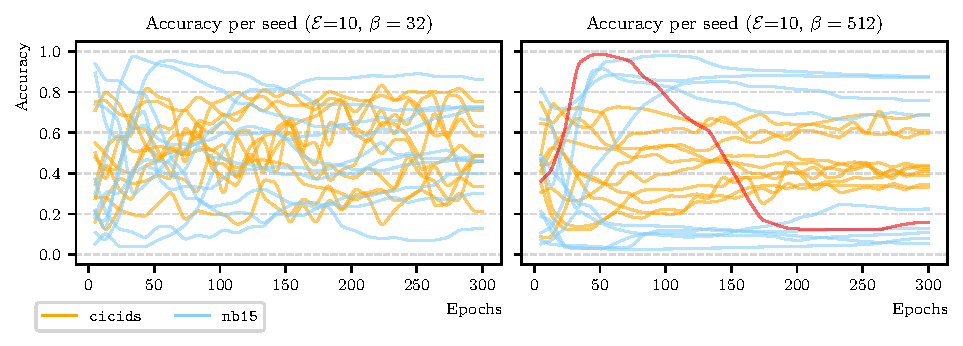
\includegraphics[width=.8\textwidth]{figures/assessment/accuracy_per_seed.pdf}
    \caption{Predictability of label-flipping attacks.}
  \end{figure}

  \begin{itemize}
    \item Very high variance in the results, but tends to stabilize (on different values) after a few rounds.

    \item The impact of the attack is highly dependent on the seed.
    \begin{itemize}
      \item[$\rightarrow$] Initial parameters, data shuffling, partitioning, \dots
    \end{itemize}
  \end{itemize}


\end{frame}

\begin{frame}{RQ2: Do Hyperparameters Influence the Impact of Poisoning Attacks?}

  \begin{figure}
    \centering
    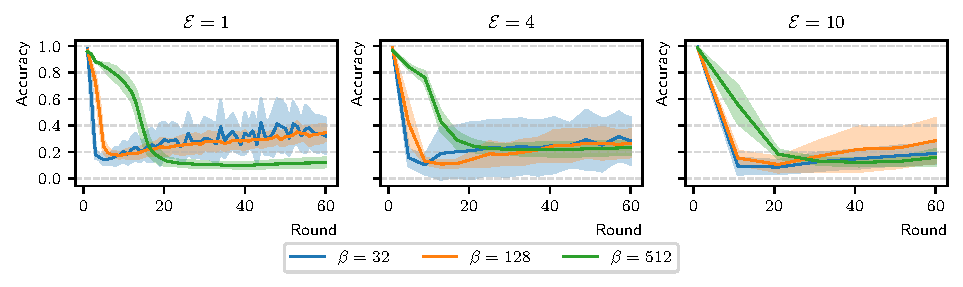
\includegraphics[width=\textwidth]{figures/assessment/hyperparams-late-icdcs.pdf}
    \caption{Effect of the hyperparameters on the accuracy of the poisoned
    model in the late scenario (50\% attackers, CICIDS).}
  \end{figure}

  \begin{itemize}
    \item \texttt{late-3} scenario: attackers start poisoning after 3 rounds
    \item High batch size leads to more inertia, less instantaneous impact
    \begin{itemize}
      \item[$\rightarrow$] More impactful in constrained environments
    \end{itemize}
  \end{itemize}

\end{frame}


\subsection*{RADAR}

\begin{frame}
  \subsectionpage
\end{frame}

\begin{frame}{Results}
  \begin{figure}
    \centering
    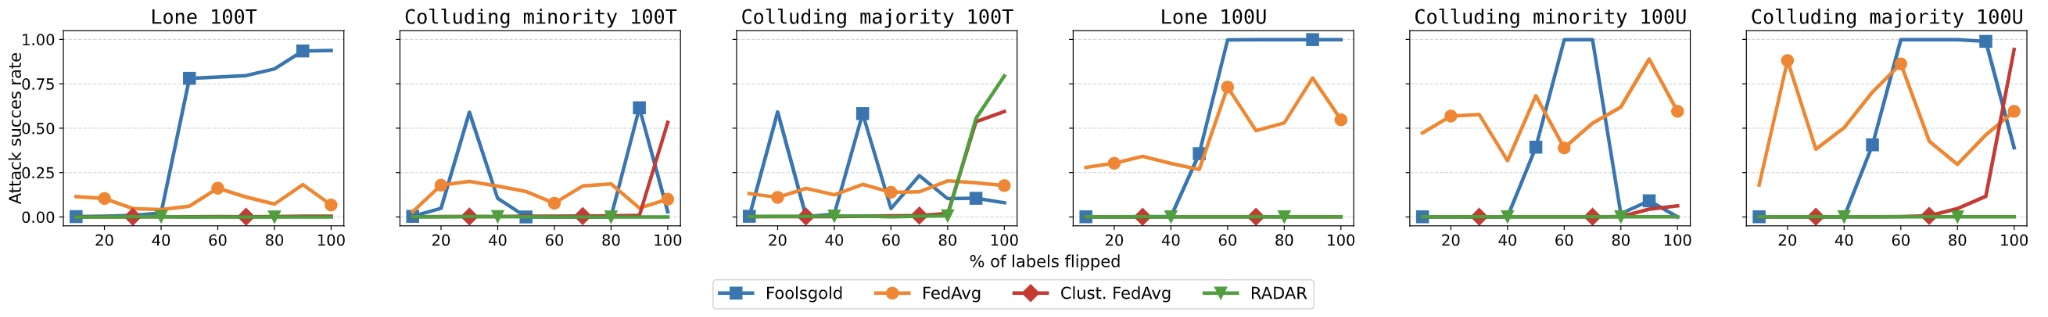
\includegraphics[width=.9\textwidth]{figures/radar/baselines.png}
    \caption{Baseline comparison.}
  \end{figure}
  \begin{figure}
    \centering
    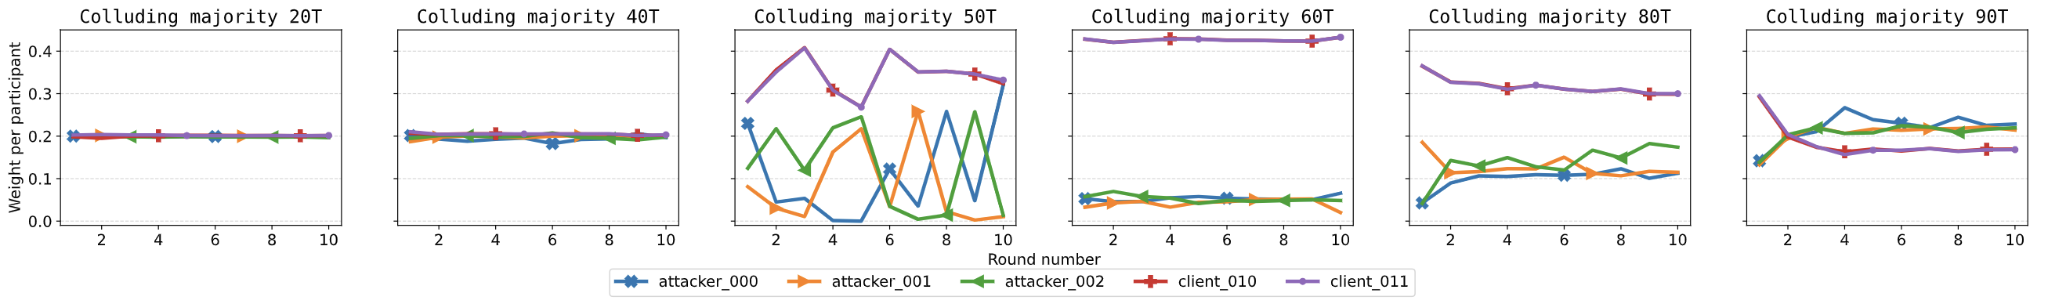
\includegraphics[width=.9\textwidth]{figures/radar/limiting-case.png}
    \caption{RADAR's limiting scenario.}
  \end{figure}
\end{frame}